\documentclass[a4paper,12pt]{article}
\usepackage[left=2.5cm, right=2.5cm, top=2.5cm, bottom=2.5cm]{geometry}
\usepackage{pdfpages}
\usepackage{amssymb}
\usepackage[backend=biber]{biblatex}
\addbibresource{../bibliography.bib}
\usepackage{minted}
\setminted{frame=lines, fontsize=\small}
\usepackage{graphicx}
\usepackage{hyperref}
\hypersetup{
    colorlinks=true,
    linkcolor=black,
    filecolor=black,
    urlcolor=black,
    citecolor=black
}
% Allow more flexible breaking of long URLs:
\setlength\emergencystretch{3em}
\setcounter{biburllcpenalty}{7000}
\setcounter{biburlucpenalty}{7000}
\Urlmuskip=0mu plus 1mu

\title{Distance-based dimensionality reduction for big data}
\author{Adrià Casanova Lloveras}

\begin{document}

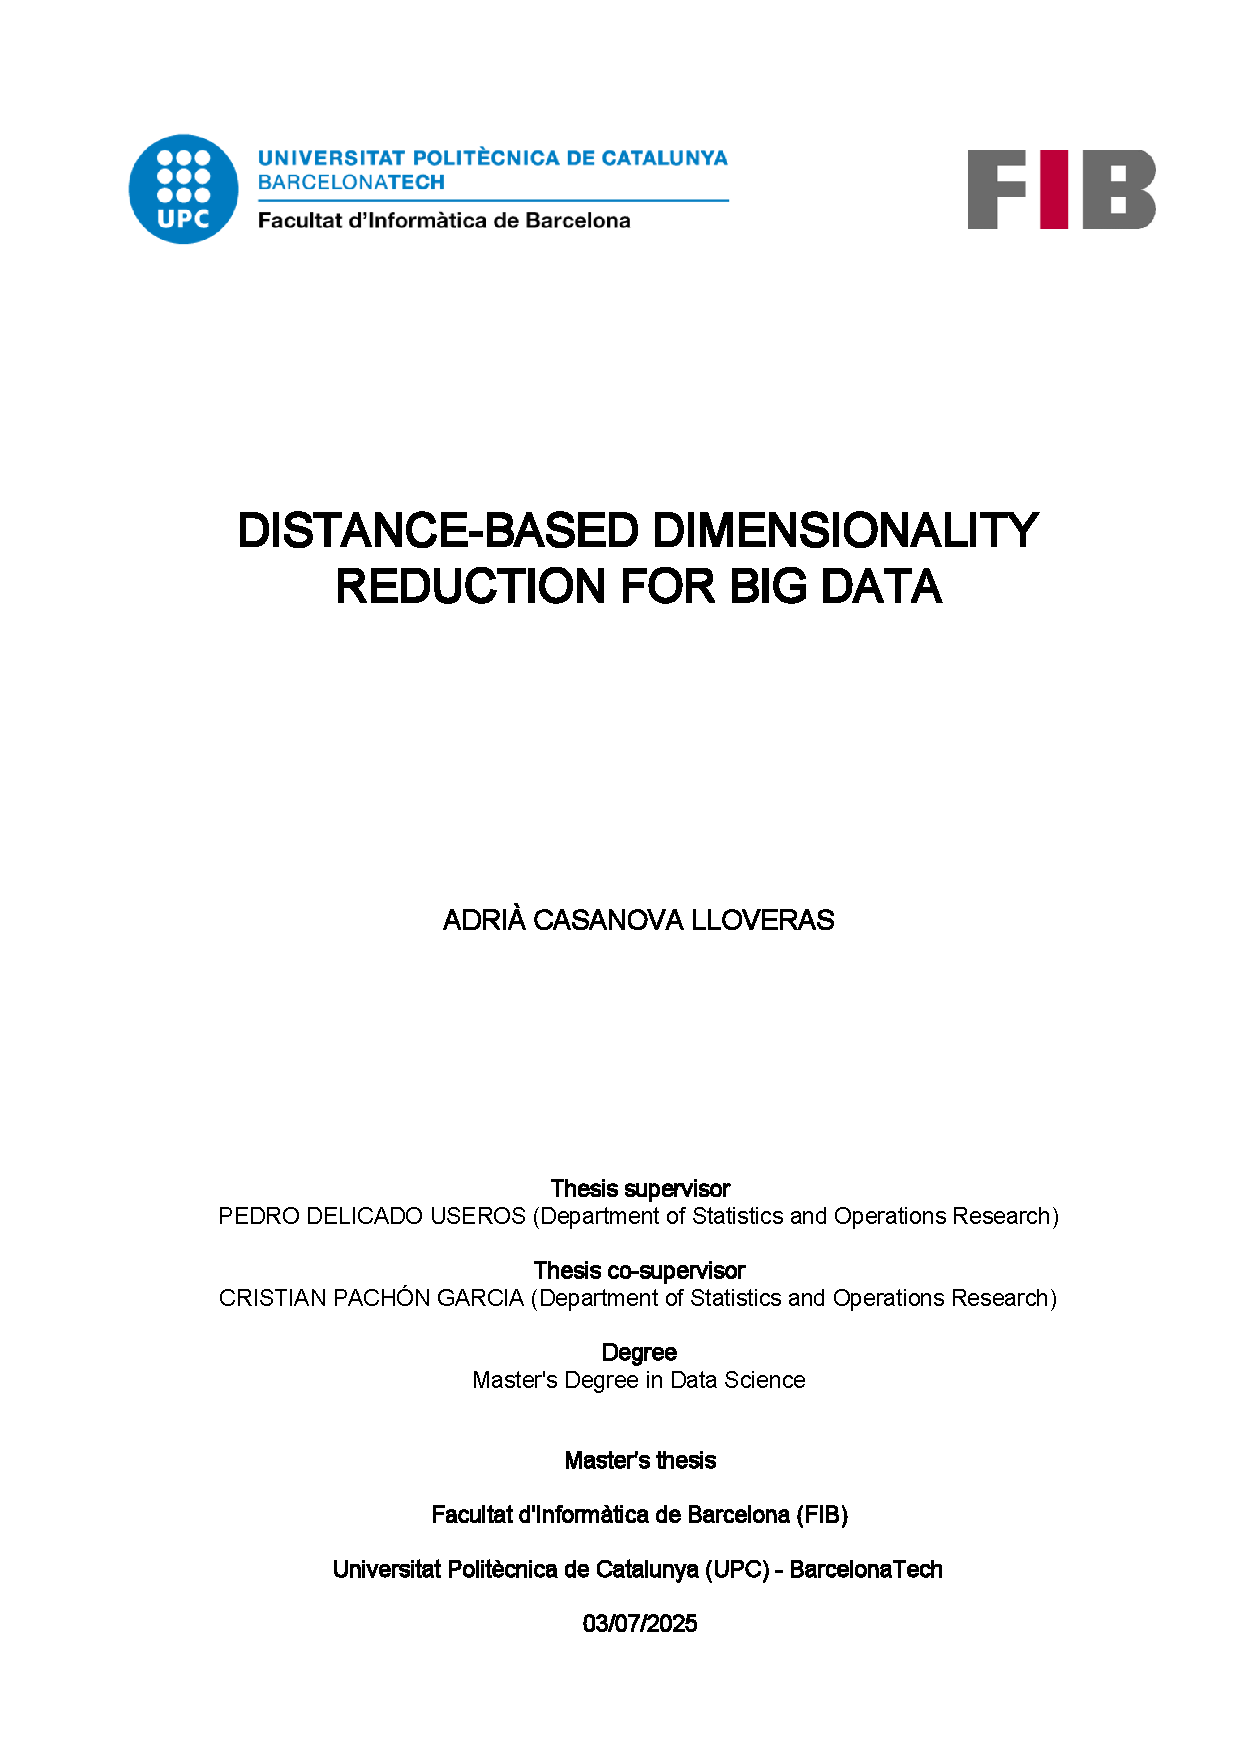
\includepdf{front_cover.pdf}

\begin{abstract}
    Example citation: \cite{Rdimtools}.
\end{abstract}
\pagebreak

\tableofcontents
\pagebreak

\section{Introduction, Motivation, and Objectives}

\subsection{Introduction}

\begin{itemize}
    \item Dimensionality Reduction definition, goal and applications.
    \item Examples of DR methods.
    \item Key points and limitations of DR methods.
\end{itemize}

\subsection{Motivation}

\begin{itemize}
    \item When the number of individuals is really large, the use of distance matrices is prohibitive.
    \item There are algorithms that extend MDS to the big data setting.
\end{itemize}

\subsection{Objectives}

\begin{itemize}
    \item Adapt these algorithms to any generic distance-based dimensionality reduction method.
\end{itemize}
\pagebreak

\section{State of the Art}

\begin{itemize}
    \item R libraries: \verb|Rdimtools|, \verb|dimRed|.
    \item \verb|bigmds| \cite{Delicado2024MDSBigData}.
    \item Landmark Isomap \cite{deSilvaTenenbaum2002}.
    \item Out-of-Core Dimensionality Reduction for Large Data via Out-of-Sample Extensions \cite{reichmann2024outofcoredimensionalityreductionlarge}.
    \item t-SNE Python implementations.
\end{itemize}
\pagebreak

\section{Specification and Design of the Solution}
\pagebreak

\section{Development of the Proposal}

\begin{itemize}
    \item DR methods descriptions.
    \item DR methods implementations.
\end{itemize}
\pagebreak

\section{Experimentation and Evaluation of the Proposal}
\pagebreak

\section{Analysis of Sustainability and Ethical Implications}

It must include an analysis of the impact of the following gender-related technical aspects:
\begin{itemize}
    \item issues related to data management and analysis
    \item issues related to equity, where possible biases are identified and assessed both in the data and in the processes carried out in relation to data management and analysis
    \item actions carried out to eliminate or mitigate such biases
\end{itemize}
\pagebreak

\section{Conclusions}
\pagebreak

\printbibliography
\pagebreak

\section{Appendices}
\pagebreak


\end{document}